\documentclass[]{beamer}

\usepackage{xeCJK}
\usepackage{fontspec}
\usepackage{graphicx}
\usepackage{animate}
\usepackage[absolute,overlay]{textpos}
\usepackage{amsthm}
\usepackage{mathtools}
%\usepackage[]{libertine}
%导入一些用到的宏包
\usepackage{amsmath,bm,amsfonts,amssymb,enumerate,epsfig,bbm,calc,color,ifthen,capt-of,multimedia,hyperref}

% Load Packages
\usepackage[utf8]{inputenc}
\usepackage{xcolor}
\usepackage{tikz}
\usetikzlibrary{positioning,calc}
\usepackage{graphicx}
\usepackage{hyperref}
\usepackage{amsmath}
\usepackage{listings}
%\usepackage{fontawesome}

% Define Commands
\newcommand*{\ClipSep}{0.06cm} %To adjust footer logo
\newcommand{\E}{\mathrm{e}\,} %\def\I{e} % used to defined e for exp(x), see later what it should be
\newcommand{\ud}{\mathrm{d}}
\lstset{numbers=left, numberstyle=\tiny, stepnumber=1,firstnumber=1,breaklines=true,
    numbersep=5pt,language=Python,
    stringstyle=\ttfamily,
    basicstyle=\footnotesize, 
    showstringspaces=false
}

\usetheme{pku}
%\usetheme{Copenhagen}

\hypersetup{
pdftitle={Network Programming},
bookmarks=true,
pdfpagemode=FullScreen
}
\title{Network Programming}
\titlegraphic{
\includegraphics[width=3cm]{Theme/Logos/logo}}
\author{}
\institute{北京大学}
\date{\today} %\today

\AtBeginSection[]
{
	\begin{frame}<beamer>
	\frametitle{\textbf{Contents}}
	\tableofcontents[currentsection]
\end{frame}
}

\beamerdefaultoverlayspecification{<+->}

\begin{document}

{\setbeamertemplate{footline}{} 
\frame{\titlepage}}

%\begin{frame}
%	\tableofcontents
%\end{frame}

\section{Connection}
\subsection{Connection}
\begin{frame}{Connection}

	\begin{itemize}
		\item 点对点: 连接一对进程
		\item 全双工: 数据同时可以在两个方向流动
		\item 可靠: 字节的发送的顺序和收到的一致
		\item 套接字(socket): 连接的端点, 地址为IP addr:port
		\item 端口(port): $16$位无符号数($2^{16}=65536$), 分为临时端口(ephermeral port)和知名端口(well-known port), 用于标识进程.
	\end{itemize}
	
	\only<6> {\centering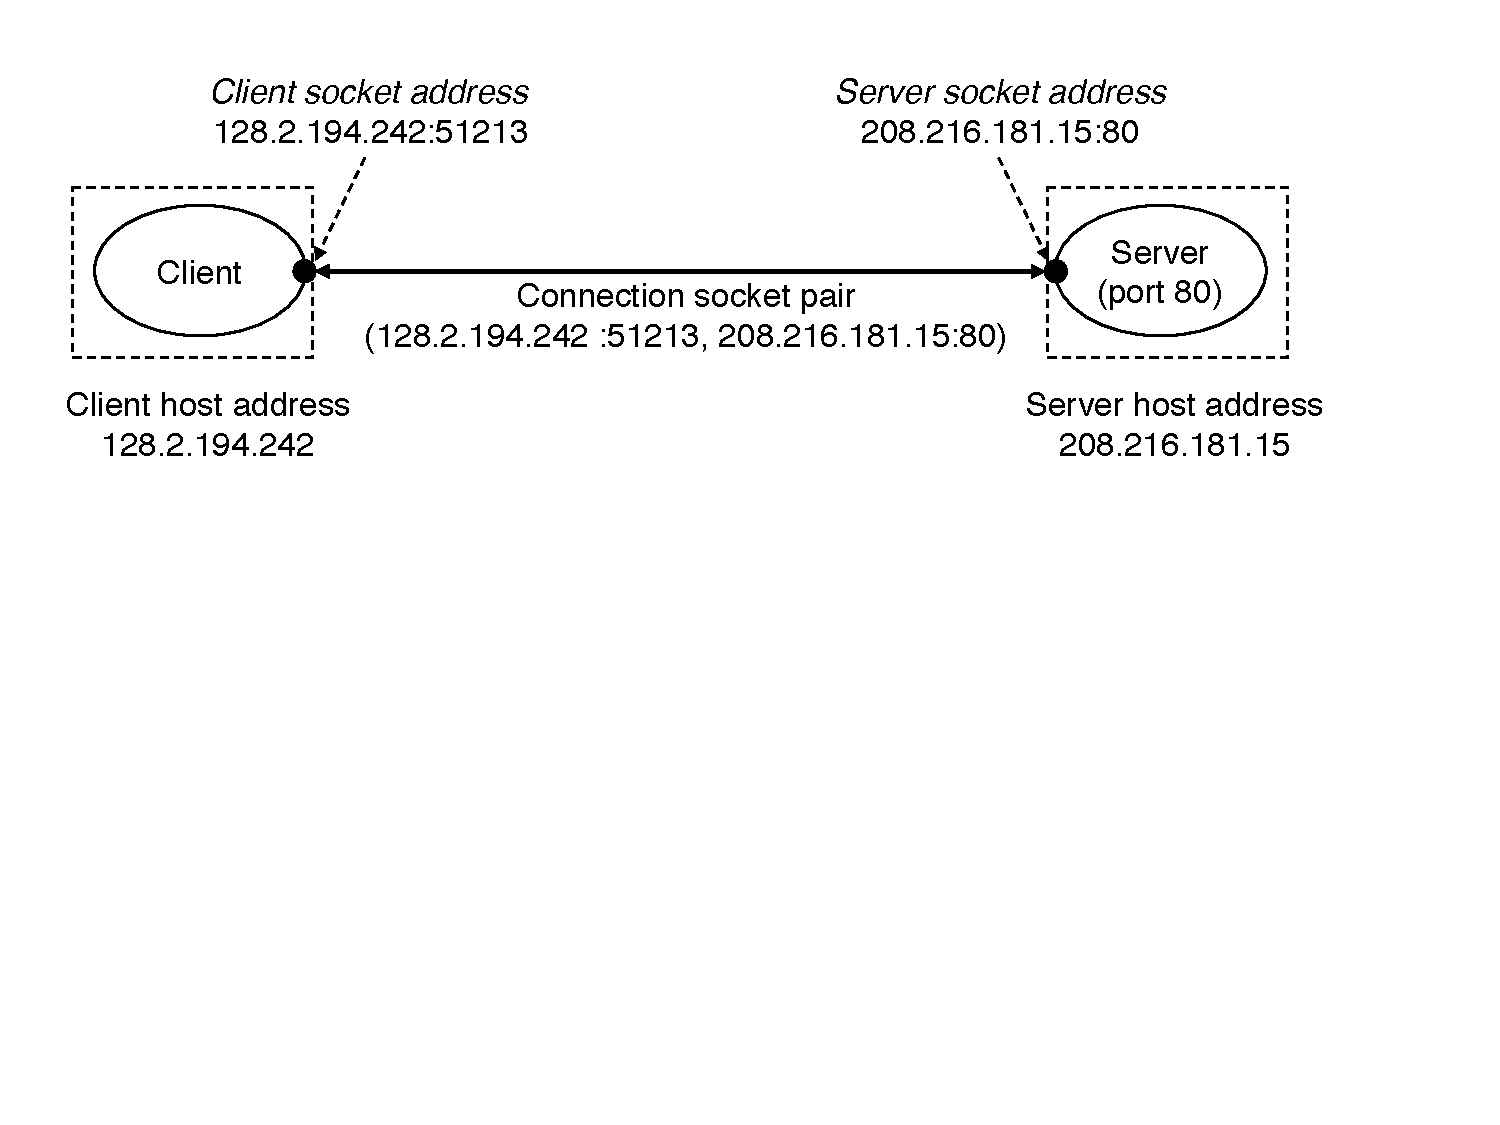
\includegraphics[width=0.8\linewidth]{figures/connection}}
	
	%\begin{block}{临时端口}
	%	连接时客户端内核自动分配
	%\end{block}
\end{frame}

\subsection{Server}
\begin{frame}{Server}
	\begin{definition}[服务器(server)]
		长时运行(守护)进程, 识别请求并处理
	\end{definition}
	
	\begin{block}{常见知名端口}
		Web(HTTP)($80$), FTP($20, 21$), SSH($22$), Telnet($23$), Mail(SMTP)($25$), HTTPS($443$)
	\end{block}
\end{frame}

\section{Echo Server}
\subsection{Overview}
\begin{frame}{Echo Server}
	将客户端发来的内容原样发回
	
	如何实现?
	\begin{enumerate}
		\item<1-> 开启服务器
		\item<1-> 开启客户端
		\item<1-> 交换数据
		\item<1-> 关闭客户端
		\item<1-> 断开客户端
	\end{enumerate}
\end{frame}

\subsection{Socket}
\begin{frame}{Socket}
	\begin{textblock*}{11.8cm}(0 cm,1.5 cm)
	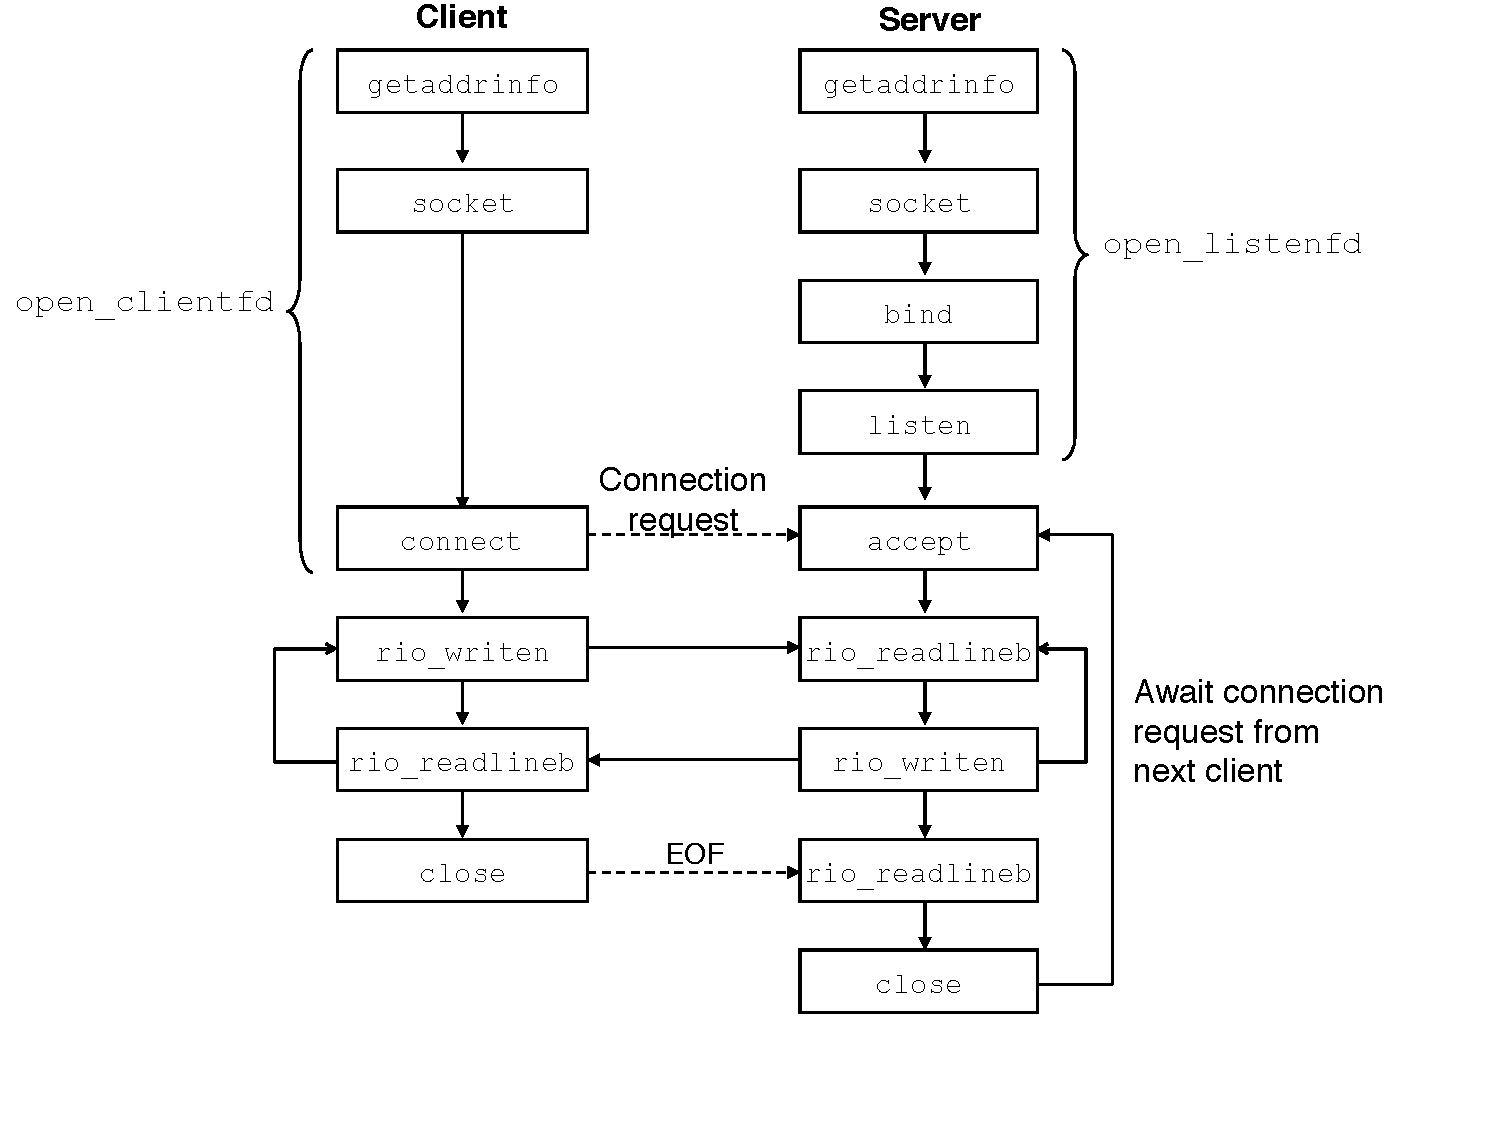
\includegraphics[width=0.7\linewidth]{figures/sockoverview}
	\end{textblock*}
	\qquad \qquad \qquad \qquad \qquad \qquad \qquad \qquad  \qquad \quad 可能考默写(18.六)
\end{frame}

\subsection{Socket Address}
\begin{frame}{Socket Address}
	IPv4 sockaddr\_in: sin\_family(AF\_INET), sin\_port, sin\_addr, sin\_zero (大端法)
	
	通用结构sockaddr: sa\_family, sa\_data
\end{frame}

\begin{frame}{\href{https://www.man7.org/linux/man-pages/man3/getaddrinfo.3.html}{getaddrinfo}}

	string $\to$ sockaddr list
	
	返回result, 其指向套接字地址链表
	
	(addrinfo), 供客户端按需访问
	
	协议无关
	
	(e.g. 不必区分IPv4/IPv6)
	
	调用后需用freeaddrinfo清理垃圾
	
	getnameinfo与之相反, 
	
	用于解析连接信息
	\begin{textblock*}{10.3cm}(7 cm,3.2 cm)
	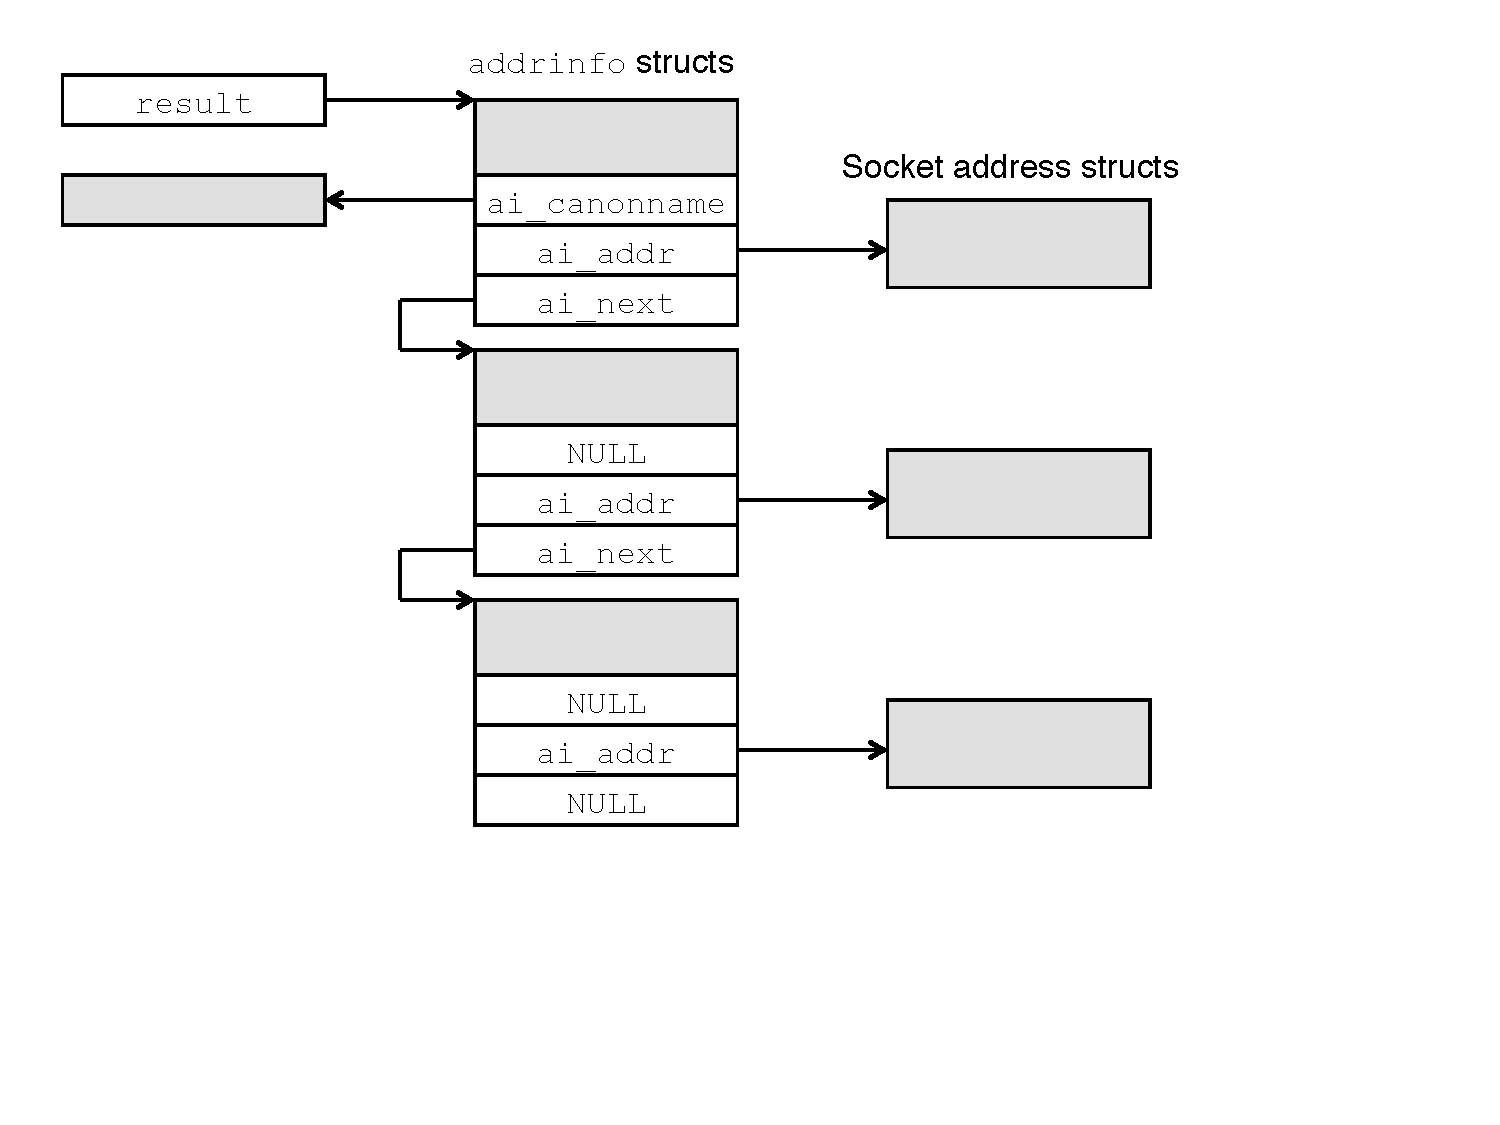
\includegraphics[width=0.58\linewidth]{figures/addrinfolist}
	\end{textblock*}
\end{frame}

\subsection{Client Side}
\begin{frame}{Client Side}
	open\_clientfd: getaddrinfo, socket(创建socket描述符), connect(建立与服务器的连接)
	
	RIOs: robust I/O for applications such as network programs that are subject to short counts
	
	close: 关闭连接
\end{frame}

\subsection{Server Side}
\begin{frame}{Server Side}
	open\_listenfd: getaddrinfo, socket, bind, listen(主动套接字$\to$监听套接字)
	
	accept: 等待并处理来自客户端的连接请求
	
	echo: 持续读写直至收到EOF
	
	监听描述符(listenfd) 已连接描述符(connfd)
\end{frame}

\begin{frame}{Quiz}
	18.一.11
	
	{\centering
	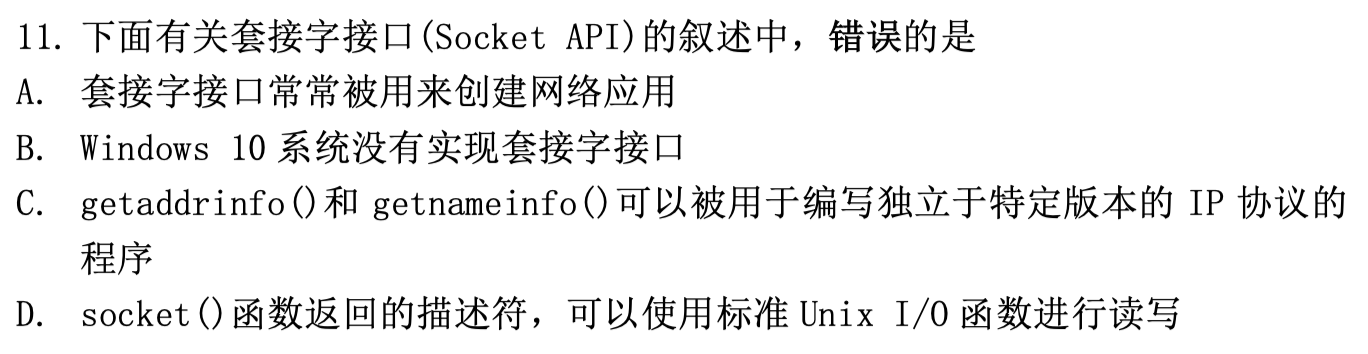
\includegraphics[width=\linewidth]{figures/2018.1}}
	
	\only<2> B
\end{frame}

\section{Web}

\subsection{Web Basics}

\begin{frame}{Web Basics}
	HTTP: 超文本传输协议
	
	MIME: html, plain, image, $\ldots$
	
	\begin{textblock*}{10.3cm}(6.5 cm,3.2 cm)
	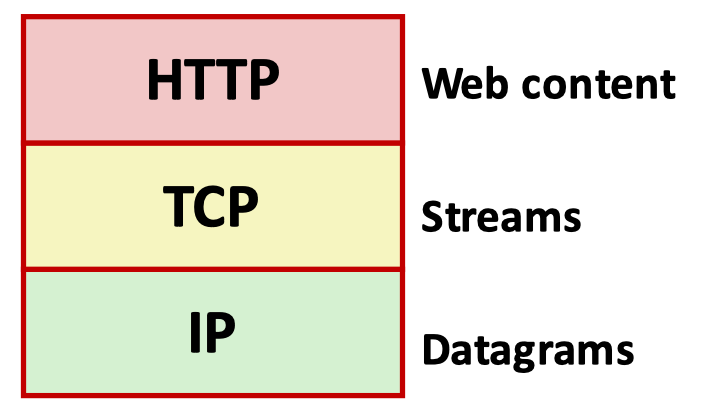
\includegraphics[width=0.6\linewidth]{figures/protocol hierachy}
	\end{textblock*}
	
	静态内容: 返回服务器上文件
	
	动态内容: 返回程序运行结果
\end{frame}

\begin{frame}{URL (通用资源定位符)}
	Static: \url{http://info.cern.ch:80/hypertext/WWW/TheProject.html}
	
	Dynamic: 
	
	\url{http://nbhbdm.cn:80/?s=\%e7\%99\%be\%e5\%ba\%a6}
	
	客户端利用前缀推断连接协议, 服务器地址和端口
	
	服务器利用后缀判断请求类型并找到相应文件, 最小后缀为"/"
	
	URI
\end{frame}

\subsection{HTTP}

\begin{frame}{HTTP Requests}
	HTTP请求$=$请求行$\times 1+$请求报头$\times k+$空行$\times 1$ 
	
	(换行使用$\backslash$r$\backslash$n)
	
	请求行$=$ method URI version
	
	method: GET, POST, \ldots
	
	请求报头$=$ header-name:header-data (e.g. User-Agent, Referer)
	
	HOST报头(HTTP/1.1): 供代理缓存使用
\end{frame}

\begin{frame}{HTTP Responses}
	HTTP响应$=$响应行$\times 1+$响应报头$\times k+$空行$\times 1+$响应主体
	
	响应行$=$ version status-code status-message

	\begin{figure}[htbp]
	\centering
	\begin{minipage}[t]{0.48\textwidth}
	\centering
	
\includegraphics[width=6cm]{figures/404}
	\end{minipage}
	\begin{minipage}[t]{0.48\textwidth}
	\centering
	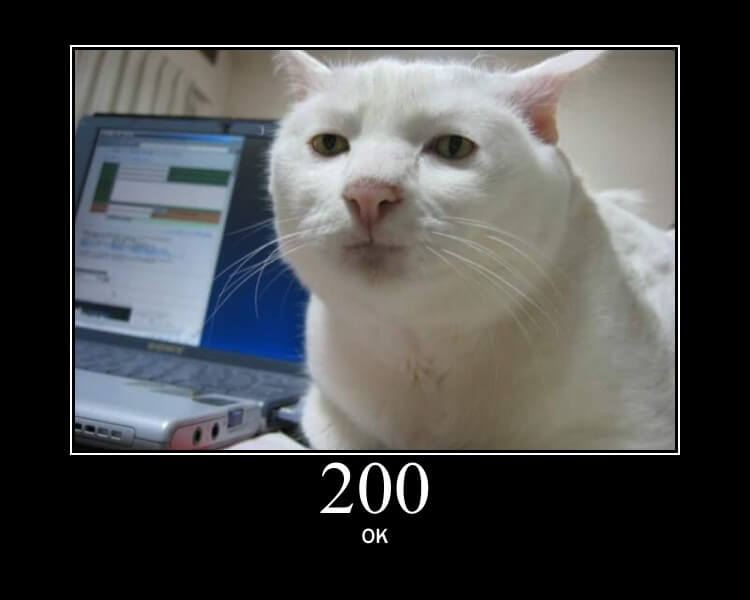
\includegraphics[width=6cm]{figures/200}
	\end{minipage}
	\end{figure}
	
	\url{https://http.cat}

\end{frame}

\begin{frame}{Serving Dynamic Content}
	服务器利用fork+execve执行子进程以应对动态请求
	
	服务器向子进程的参数传递遵循CGI(通用网关接口)
	
	重定向标准输出到已连接描述符
	
	\begin{alertenv}
		子进程要负责输出Content-type, Content-length响应报头及空行.
	\end{alertenv}
	
\end{frame}

\begin{frame}{Serving Dynamic Content}
	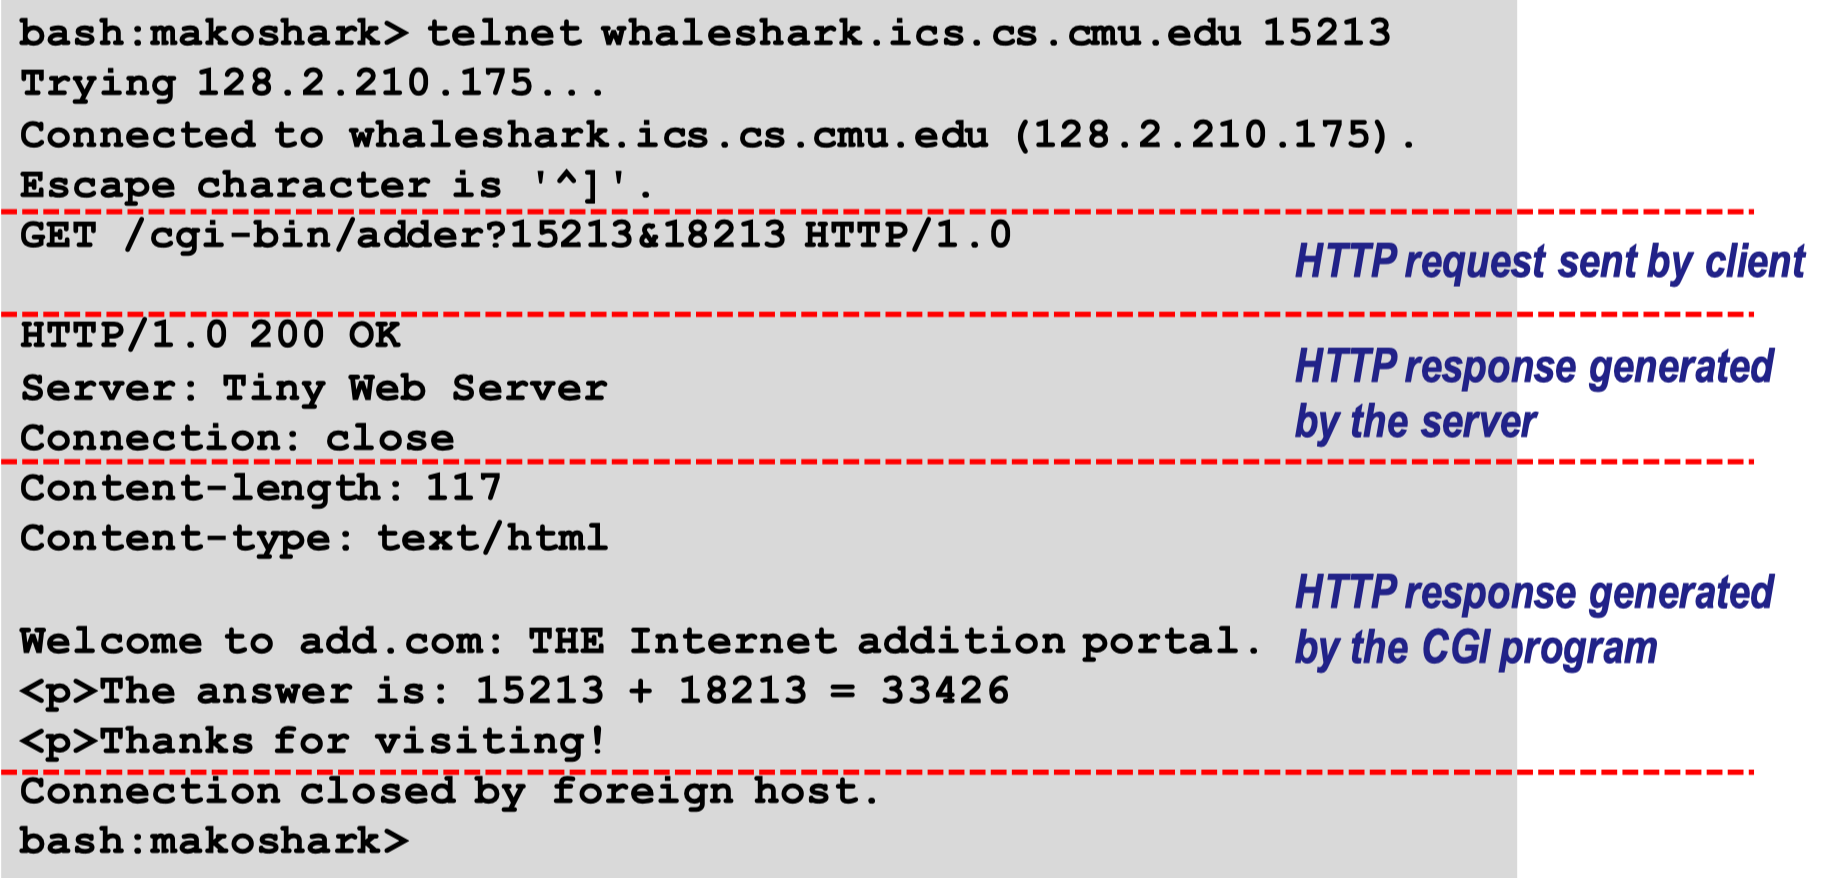
\includegraphics[width=\linewidth]{figures/dynamic}
\end{frame}

\subsection{Proxy}
\begin{frame}{Proxy}
	客户端 $\rightleftharpoons$ 代理服务器 $\rightleftharpoons$ 原始服务器
	
	优点: 提高访问速度(利用缓存), 控制对内部资源的访问, 过滤内容, 隐藏真实IP(e.g. Tor), 突破内容过滤机制限制(GFW), 转码
	
	\only<2->{
	\begin{block}{显式代理}
		客户端显式配置使用代理,此时客户端知道正向代理的存在
		
		请求需给出完整URL
	\end{block}
	}
	
	\only<3->{
	\begin{block}{透明代理}
		客户端没有进行任何配置,不知道代理的存在, 代理在中途拦截并完成请求
	\end{block}
	}

\end{frame}

\section{Exam review}

\begin{frame}{Exam Review}

	数连接最大值, 端口(13.七, 14.八)
	
	socket连接过程(13.七, 14.八, 18.六)
	
	connection socket pairs的合法性判断/书写(13.一.18)
	
	写代码(16.七, 实现基于进程的并发echo server, 补全open\_listenfd)
	
	静态/动态内容的概念(14.八, 15.一.17) 
	
	与并发编程的联系
\end{frame}

\begin{frame}
\begin{center}
   \LARGE{谢谢!}
\end{center}
\end{frame}

\end{document}

